\chapter{Clustering} % (fold)
\label{cha:clustering}

Il clustering può essere considerato il più importante problema di \textbf{apprendimento non supervisionato} in quanto trova innumerevoli applicazioni in svariati campi del sapere. L’obiettivo che si pone è organizzare dati non classificati in gruppi, i cui membri sono simili per un qualche criterio. Un \textbf{cluster} è quindi una collezione di oggetti che sono simili tra di loro, e dissimili dagli oggetti appartenenti ad altri cluster. Formalmente:

\begin{mydef}[Problema del clustering]
	Dati $n$ oggetti e una matrice di similarità $n \times n$ lo scopo è partizionare gli inputs in gruppi massimalmente omogenei (i.e \textbf{clusters}).
\end{mydef}

Il criterio di similarità che deve essere fornito per poter fare un clustering dei dati può essere visto come una funzione $\phi$ che dati due oggetti ritorna la loro similarità. Questa misura è \emph{simmetrica} se per una qualunque coppia di oggetti $(a, b)$ abbiamo che $\phi(a, b) = \phi(b, a)$ altrimenti è \emph{asimmetrica}.\\

\begin{figure}[h!]
	\centering
	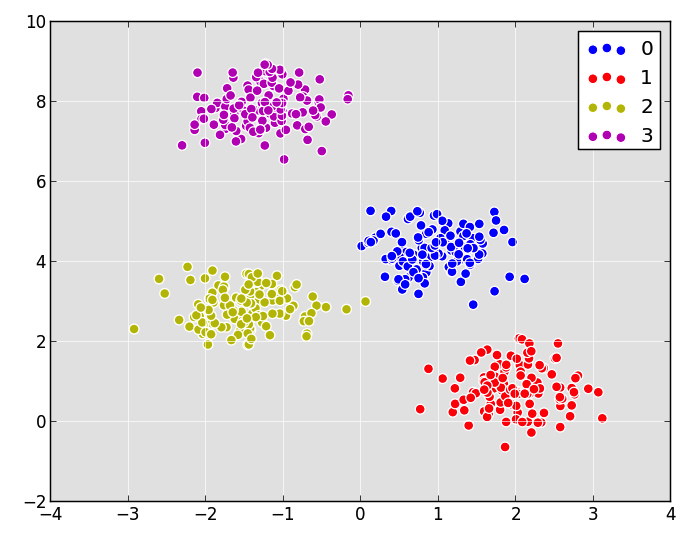
\includegraphics[width=8cm]{images/clustering.png}
	\caption{Esempio di clustering}\label{fig:clusters}
\end{figure}

In questo esempio è possibile identificare quattro cluster nei quali possono essere suddivisi i dati e il criterio di similarità usato è la \emph{distanza}, quindi due oggetti fanno parte di uno stesso cluster solo se sono sufficientemente vicini tra di loro. 

\newpage

Questo tipo di clustering è detto \emph{distance-based}, ovvero basato sulla distanza. In generale, a seconda del tipo di input il problema del partizionamento si divide in:
\begin{enumerate}
	\item \textbf{feature-based:} gli oggetti sono rappresentati come vettori di caratteristiche. Nella letteratura l'algoritmo più noto è il \emph{k-means};
	\item \textbf{pairwise:} è sufficiente solo una matrice di similarità tra tutte le coppie di oggetti; non è necessario avere la rappresentazione vettoriale degli oggetti, si tratta quindi di un approccio più generale rispetto al primo. Una degli algoritmi più popolari è il \emph{normalized cut (ncut)}. 
\end{enumerate}

Non sempre è facile ed intuitivo trovare un raggruppamento per i dati, come invece lo era per l’esempio visto, in quanto è difficile stabilire cosa costituisce un “buon clustering” e cosa no. In generale si può affermare che un cluster deve soddisfare i seguenti criteri:
\begin{itemize}
	\item \textbf{criterio interno}: tutti gli oggetti all'\emph{interno} di un cluster devono essere il più possibile simili tra loro;
	\item \textbf{criterio esterno}: tutti gli oggetti all'\emph{esterno} di un cluster devono essre il più possibile dissimili rispetto a quelli contenuti al suo interno.
\end{itemize}

Nelle sezioni seguenti saranno presentati tre metodi di clustering:  K-Means, N-Cut e insiemi dominanti. Il primo è di tipo feature-based, mentre i rimanenti sono entrambi di tipo pairwise, ma utilizzano tecniche differenti. In particolare N-Cut è basato sulla teoria spettrale dei grafi, mentre gli insiemi dominanti utilizzano metodi della teoria dei giochi per affrontare il problema.

\newpage

\section{K-Means} % (fold)
\label{sec:k_means}
K-Means è probabilmente il più famoso algoritmo di partizionamento. Dato un insieme di osservazioni $\{x^{(1)},\dots,x^{(n)} \}$ dove $x_i$ è un vettore m-dimensionale, lo scopo dell'algortimo è partizionare l'insieme in $k$ insiemi $k \leq n$ il più possibile coesi tra loro (problema del clustering).\\

L'algoritmo k-means seleziona a caso $k$ prototipi, ciascuno di essi rappresenta il proprio gruppo di appartenzenza, idealmente il centro del cluster. Formalmente si introduce un insieme di vettori:
\begin{align*}
	\mu_j, \text{ dove } j = 1, \dots, k
\end{align*}
L'obiettivo ora consiste nel raggruppare le osservazioni e assegnare i vettori $\mu_j$ in modo tale che la somma del quadrato delle distanze da un punto al proprio centroide $\mu_j$ sia minima. In termini matematici si tratta di minimizzare la seguente funzione:
\begin{align}
	\min_{\{\mu_1, \dots, \mu_k\}} \sum_{i=1}^n \sum_{j=i}^k r_{ij} \| x_i - \mu_j \|^2\label{eq:j}
\end{align}
dove $r_{ij}$ è un operatore binario $r_{ij} \in \{ 0, 1 \}$. In fase di inizializzazione, si scelgono $k$ punti casuali come centri e in seguito si esegue una procedura iterativa per minimizzare \eqref{eq:j}. Ogni iterazione si compone di \textbf{due} fasi: nella prima fase (\emph{Expectation-Step}) si minimizza rispetto a $r_{ij}$ mantenendo $\mu_j$ fisso, mentre nella seconda fase (\emph{Maximization-Step}) si minimizza rispetto a $\mu_j$ mantenendo $r_{ij}$ fisso. Formalmente, nella fase E, il calcolo di $r_{ij}$ è dato da:
\begin{align*}
	r_{ij} =
	\begin{cases}
		1, &\text{ se }j = argmin_j \| x_i - \mu_j \|^2 \\
		0, &\text{ altrimenti}
	\end{cases}
\end{align*}
Intuitivamente si assegna l’osservazione $x_i$ al gruppo con $\mu_j$ più vicino.

\newpage

Nella seconda fase $\mu_k$ è dato da:

\begin{align*}
	\mu_j = \frac{\displaystyle\sum_i r_{ij} x_i}{\displaystyle\sum_i r_{ij}}
\end{align*}

Ovvero, si cerca di “spostare” al centro del cluster il prototipo $\mu_j$ come la media di tutti i punti $x_i$ assegnati al cluster $k$. Queste due fasi si ripetono fino a quando non c'è più alcuna variazione negli assegnamenti o quando un numero massimo di iterazioni è raggiunto. Infatti, trattandosi di un problema NP-Difficile non è dato sapere a priori se l'algoritmo converga oppure no.

\begin{figure}[h!]
    \centering
	\subfigure{
    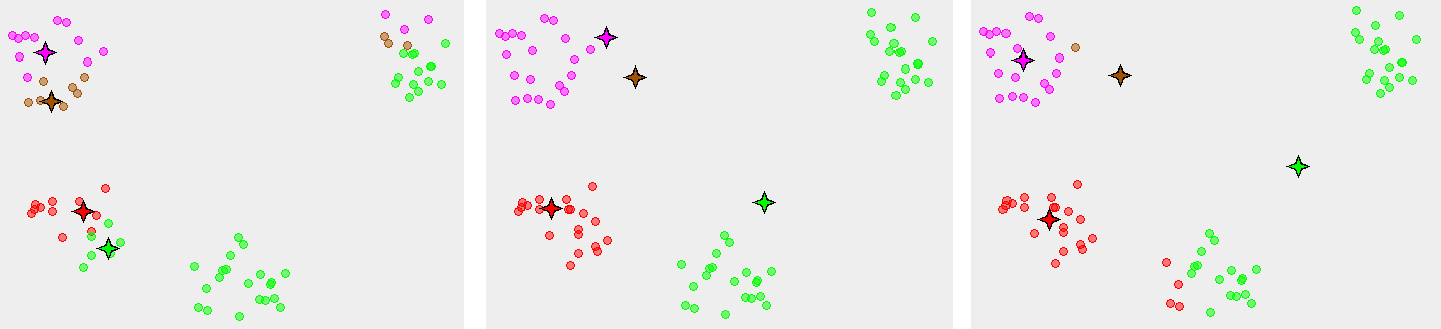
\includegraphics[width=12cm]{images/kmeans}
	}
	\subfigure{
    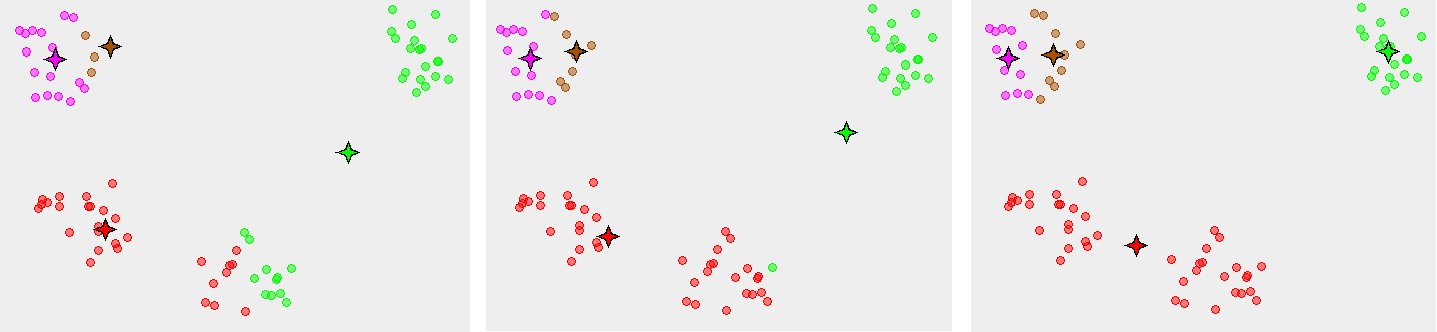
\includegraphics[width=12cm]{images/kmeans2}
	}
	\caption{Esempio sulla convergenza (dopo 5 iterazioni) a un minimo locale dell'algoritmo k-means}
\end{figure}

% section k_means (end)


\section{Normalized Cut} % (fold)
\label{sec:normalized_cut}
A differenza del k-means l'algoritmo presentato in questa sezione è basato sulla teoria dei grafi e trova ampio utilizzo nella \emph{segmentazione delle immagini}, un problema analogo al clustering.
L'algoritmo \emph{normalized cut} “taglia” l'immagine utilizzando tecniche della \textbf{teoria spettrale} dei grafi. Un buon taglio divide pixel che sono dissimili tra loro. Per trovare un buon partizionamento l'algoritmo segue i seguenti passi:
\begin{enumerate}
	\item Si costruisce un grafo di similarità $G=(V, E, w)$ in cui ogni nodo rappresenta un pixel dell'immagine e il peso su ciascun arco rappresenta una misura di similarità (intensità, colore ecc..) tra ciascun pixel.
	\item Si calola il Laplaciano normalizzato definito come:
	\begin{align}
		L = D ^ {- 1 / 2} (D - A) D ^ {- 1 / 2}
	\end{align}
	dove $A$ è la matrice di adiacenza pesata e $D$ è la matrice dei gradi così definita:
	\begin{align}
		d_{i,j}:=
		\begin{cases} 
		\deg(v_i) & \mbox{if}\ i = j \\
		0 & \mbox{otherwise}
		\end{cases}
	\end{align}
	Si calcolano gli autovettori del Laplaciano normalizzato:
	\begin{align}
		L x = \lambda x
	\end{align}
	
	\item Utilizzando il segno nel secondo autovettore più piccolo (il primo è un vettore nullo) si segmenta l'immagine in due parti.

	\item La procedura si ripete ricorsivamente su ciascun segmento dell'immagine per $n$ volte.
\end{enumerate}

L'algoritmo nella pratica si è dimostrato abbastanza efficace tuttavia il calcolo degli autovettori è un problema computazionalmente costoso: $O(n^3)$ dove $n$ è il numero di pixel. L'algoritmo diventa quindi impraticabile per immagini di dimensioni eccessive.\\

\begin{figure}[h!]
    \centering
	\subfigure[$original$]
	{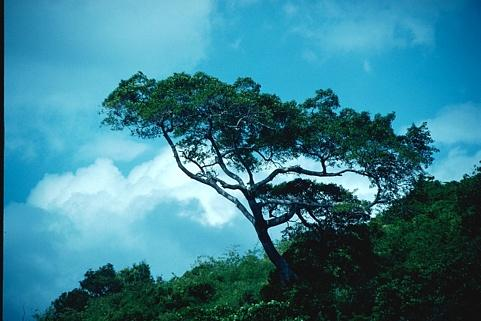
\includegraphics[width=3cm]{images/0.jpg}}
	\subfigure[$k = 2$]
	{
\includegraphics[width=3cm]{images/1.png}}
	\subfigure[$k = 3$]
	{
\includegraphics[width=3cm]{images/2.png}}
	\subfigure[$k = 4$]
	{
\includegraphics[width=3cm]{images/3.png}}
	\caption{Esempio di segmentazione ottenuta con NCUT.}
\end{figure}


% section normalized_cut (end)

\newpage

\section{Insiemi dominanti} % (fold)

Prima di presentare il concetto di insieme dominante è necessario introdurre il \emph{problema della cricca massima}. Si vedrà, infatti, che un insieme dominante non è altro che una \textbf{clique massimale} di un grafo.

\subsection{Problema della cricca massima} % (fold)
\label{ssec:problema_della_cricca_massima}
Sia $G=(V,E)$ un grafo non orientato con $V$ l'insieme dei vertici ed $E$ quello degli archi, tale per cui $V={1,\dots,n}$ e $E \subseteq V \times V$. Si definisce cricca (o clique) $C \subseteq V$, un sottoinsieme di vertici di G che formano un grafo completo, ovvero tale che $\forall i,j \in C$ con $i \neq j, (i,j) \in E$.

\begin{mydef}[Clique massimale]
Si definisce \textbf{clique massimale} di $G$ una clique di $G$ che non è contenuta in nessun'altra clique di $G$.    
\end{mydef}

\begin{mydef}[Clique massima]
    Si definisce \textbf{clique massima} di $G$ una clique massimale di G di cardinalità massima.
\end{mydef}
Il problema consiste nel trovare una cricca massimale (MCP). Ad esempio si consideri il seguente grafo:

\begin{figure}[h!]
    \centering
    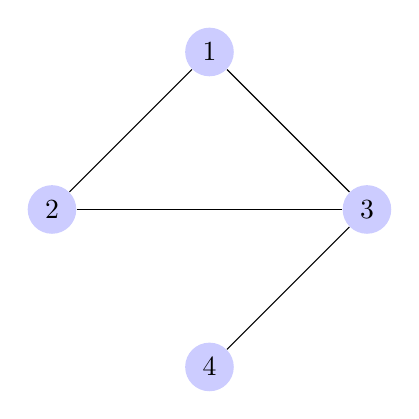
\begin{tikzpicture}
        \node[circle,fill=blue!20] (1) at (0,2) {1};
        \node[circle,fill=blue!20] (2) at (-2,0) {2};
        \node[circle,fill=blue!20] (3) at (2,0) {3};
        \node[circle,fill=blue!20] (4) at (0, -2) {4};
    
        \foreach \from / \to in {1/2,2/3,1/3,3/4}
            \path (\from) edge (\to);
    \end{tikzpicture}
    \caption{Un grafo non orientato.}\label{fig:graph1}
\end{figure}
Le clique nel grafo sono:
\begin{align*}
    C_1 &= \{1,2\} \tag{$C_1$ non è massimale perché $C_1 \subseteq C_2$}\\
    C_2 &= \{1,2,3\} \tag{Massimale e massima}\\
    C_3 &= \{3,4\} \tag{Massimale}
\end{align*}

\newpage

Trovare la cricca massimale è un problema facile, mentre trovare quella massima è NP-difficile, così come trovare la dimensione di tale clique. In questa sezione si affronta il problema sotto quest'ultimo punto di vista.\\

Per affrontare il problema con le reti neurali è necessario trasformare MCP da problema discreto a problema continuo. Nell'esempio del TSP con il modello di Hopfield, non è detto che ci sia il percorso inverso (potremo ottenere ad esempio una matrice che non ha significato); in questo nuovo problema MCP, la bidirezionalità è d'obbligo.\\

Si utilizza quindi un nuovo approccio, ma prima sono necessarie alcune notazioni:
\begin{itemize}
    \item Se $C \subseteq V$, $x^C$ indica il \textbf{vettore caratteristico} definito come:
    \begin{align*}
        x^C_i = 
        \begin{cases}
            \displaystyle\frac{1}{|C|}, &\text{se }i \in C\\
            0,  &\text {altrimenti}
        \end{cases}
    \end{align*}
    dove $|C|$ indica la cardinalità dell'insieme $C$ e $i \in \{ 1, \dots, |V|\}$
    \item $S_n$ è il \textbf{simplesso standard} in $\mathbb{R}^n$:
    \begin{align*}
        S_n = \left\{x \in \mathbb{R}^n : \sum_{i=1}^n x_i = 1 \text{ e } x_i \geq 0, \forall i \right\}
    \end{align*}
    Per qualunque vettore caratteristico vale la relazione $x^C \in S_n$ con $n \geq |C|$
    \item $A=(a_{ij})$ è la matrice di adiacenza di $G$:
    \begin{align*}
        a_{ij} =
        \begin{cases}
            1, &\text{ se } (i,j) \in E \\
            0, &\text{ altrimenti}
        \end{cases}
    \end{align*}
\end{itemize}


\newpage

\begin{figure}[h!]
    \centering
    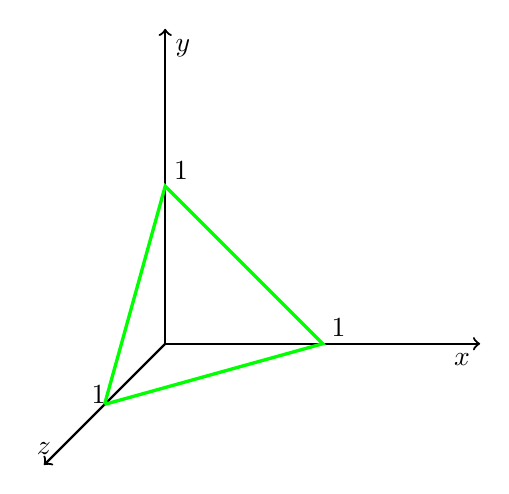
\begin{tikzpicture}[scale=2]

        %draw the main coordinate system axes
        \draw[thick,->] (0,0,0) -- (2,0,0) node[anchor=north east]{$x$};
        \draw[thick,->] (0,0,0) -- (0,2,0) node[anchor=north west]{$y$};
        \draw[thick,->] (0,0,0) -- (0,0,2) node[anchor=south]{$z$};
        
        \draw[thick, color=green, very thick] plot coordinates{(0,0,1) (0,1,0) (1,0,0) (0,0,1)};
        
        \node at (1.1,0.1,0) {1};
        \node at (0.1,1.1,0) {1};
        \node at (0,0.1,1.1) {1};
        
    \end{tikzpicture}
    \caption{Rappresentazione grafica del simplesso standard}
\end{figure}

Si consideri la seguente funzione quadratica continua in $n$ variabili:
\begin{align*}
    &f_G(x) = x^T A x = \sum_{i=1}^n \sum_{j=1}^n a_{ij} x_i x_j \tag{Lagrangiano del grafo} \\
    &\text{oppure } f_G(\bar{x}) = \sum_{(i,j) \in E} x_i x_j
\end{align*}
dove $x^T$ è il vettore trasposto e $A$ è la matrice di adiacenza. Ad esempio se si considera il grafo in Figura~\ref{fig:graph1} allora:
\begin{align*}
    f_G(x) = x_1 x_2 + x_1 x_3 + x_2 x_3 + x_3 x_4
\end{align*}

\subsubsection{Teorema di Motzkin-Strauss} % (fold)
Si è detto che per affrontare MCP con le reti neurali è necessario fornire una formulazione continua del problema. A tale scopo si introduce il teorema di Motzkin-Strauss.
\begin{thm}[Teorema di Motzkin-Strauss]
    Sia $x^*$ un massimo globale di $f_G$ in $x \in S_n$ allora la cardinalità della clique massima è legata a $f_G(x)$  dalla seguente formula:
    \begin{align*}
           \omega(G) = \frac{1}{1 - f(x^*)}
    \end{align*}
    Inoltre un sottoinsieme di vertici $C$ è una clique massima se e solo se il suo vettore caratteristico $x^C \in S_n$ è un massimo globale per $f_G$ in $S_n$.
\end{thm} 
\newpage

Il teorema di Motzkin-Strauss fornisce una connessione tra la cardinalità della clique massima $\omega(G)$ di un grafo $G$ con $n$ vertici e il massimo del suo Lagrangiano definito nel simplesso standard di $\mathbb{R}^n$. In particolare è stato mostrato che una clique $C$ è massima se e solo se il suo vettore caratteristico $x^C$ è un massimizzatore globale della funzione $f_G$ su $S_n$.\\

Tuttavia non tutti i massimizzatori di $f_G$ sono nella forma di vettori caratteristici e pertanto non possono essere utilizzati direttamente per ricavare informazioni sulle clique massime. Tali massimizzatori sono definiti \emph{soluzioni spurie}. Ad esempio, si consideri il seguente grafo:

\begin{figure}[h!]
    \centering
    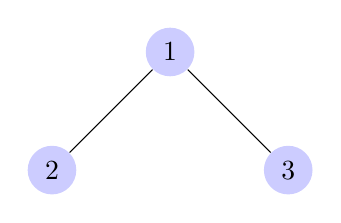
\begin{tikzpicture}
        \node[circle,fill=blue!20] (1) at (0,1.5) {1};
        \node[circle,fill=blue!20] (2) at (-1.5,0) {2};
        \node[circle,fill=blue!20] (3) at (1.5,0) {3};
        
        \draw (1) -- (2);
        \draw (1) -- (3);
        
    \end{tikzpicture}
    \caption{Grafo esempio.}
\end{figure}
 Il grafo presenta due massimi globali:
 \begin{align*}
     C_1 = \{1,2\} \qquad  x^{C_1} = (1 / 2, 1 / 2, 0) \\
     C_2 = \{1,3 \} \qquad x^{C_2} = (1 / 2, 0, 1 / 2)
 \end{align*}

Tuttavia come si evince dal seguente grafico, sono massimi globali anche tutti i punti del segmento $x'x''$ ovvero tutti i punti in $(1/2, \alpha / 2, (1 - \alpha) / 2) \, \forall \alpha \in [0,1]$.
\begin{figure}[h!]
    \centering
    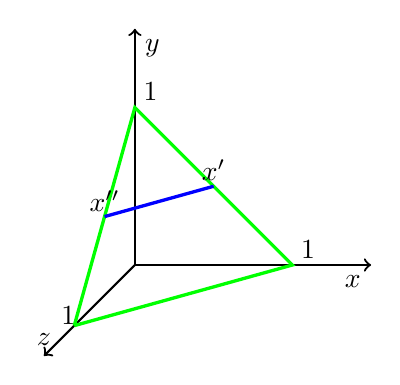
\begin{tikzpicture}[scale=2]
        %draw the main coordinate system axes
        \draw[thick,->] (0,0,0) -- (1.5,0,0) node[anchor=north east]{$x$};
        \draw[thick,->] (0,0,0) -- (0,1.5,0) node[anchor=north west]{$y$};
        \draw[thick,->] (0,0,0) -- (0,0,1.5) node[anchor=south]{$z$};
        
        \draw[thick, color=green, very thick] plot coordinates{(0,0,1) (0,1,0) (1,0,0) (0,0,1)};
        \draw[color=blue, very thick] (.5, .5, 0) -- (0,.5,.5);
        
        \node at (.5,.6,0) {$x'$};
        \node at (0,.6,.5) {$x''$};
        
        \node at (1.1,0.1,0) {1};
        \node at (0.1,1.1,0) {1};
        \node at (0,0.1,1.1) {1};
        
    \end{tikzpicture}
    \caption{Soluzioni spurie in MCP}
\end{figure}

Dunque $x'$ e $x''$ \textbf{non} sono vettori caratteristici e non possono essere utilizzati per la soluzione del MCP.

\newpage

Quello che è stato fatto finora è prendere il problema $P$ di clique massima nel discreto e trasformarlo in un problema $P'$ di ottimizzazione quadratica nel continuo. A questo punto è necessario mappare la soluzione del problema $P'$ in una soluzione del problema originale $P$.  Questo è possibile se la soluzione ottenuta in $P'$ è un vettore caratteristico.\\

Il problema delle soluzioni spurie è stato recentemente risolto da Bomze (1995) proponendo una versione regolarizzata di $f_G(x)$. La soluzione consiste nel sommare $1/2$ alla diagonale principale della matrice di adiacenza $A$.
\begin{align*}
    A' = A + \frac{1}{2} I
\end{align*}
Da cui si ottiene:
\begin{align*}
    \hat{f}_G(x) = x^T A' x = x^T \left( A + \frac{1}{2} I \right) x 
\end{align*}
Dove I è la matrice identità, ovvero una matrice quadrata dello stesso lato di $A$ con tutti gli elementi in diagonale principale ad 1 e tutti gli elementi al di fuori di essa a 0.\\


\begin{figure}[h!]
    \centering
    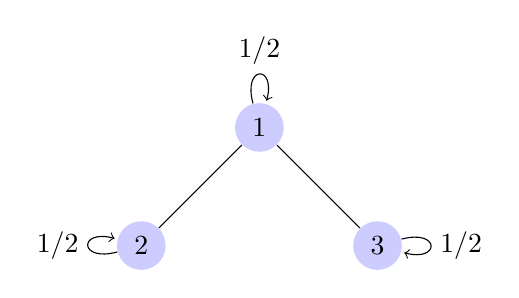
\begin{tikzpicture}
        \node[circle,fill=blue!20] (1) at (0,1.5) {1};
        \node[circle,fill=blue!20] (2) at (-1.5,0) {2};
        \node[circle,fill=blue!20] (3) at (1.5,0) {3};
        
        \path
		(1) edge (2)
		(1) edge (3)
		(1) edge[loop above] node{$1/2$} (1)
		(2) edge[loop left] node{$1/2$} (2)
		(3) edge[loop right] node{$1/2$} (3)
		;
        
    \end{tikzpicture}
    \caption{Soluzione problema delle soluzioni spurie (Bomze).}
\end{figure}

Riassumendo il problema della cricca massima dato un grafo $G = (V, E)$ è definito nel seguente modo:
\begin{align*}
	\max(\hat{f}_G(x)) \text{ tale che } x \in S_n
\end{align*}
Sia $C \subseteq V$ e sia $x^C$ il suo vettore caratteristico allora:
\begin{enumerate}
	\item $C$ è una clique massima di $G$ sse $x^C$ è un massimo globale di $\hat{f} \in S_n$;
	\item $C$ è una clique massimale di $G$ sse $x^C$ è un massimo locale di $\hat{f} \in S_n$;
	\item ogni massimo locale è un vettore caratteristico ed è locale stretto. 
\end{enumerate}

% subsection problema_della_cricca_massima (end)


\label{subsec:Definizione di insieme dominante}
Dato un grafo pesato indiretto $G = (V, E , w)$ dove $V = \{ 1, \dots, n \}$ è l'insieme dei vertici, $E \subseteq V \times V$ l'insieme degli archi e $w : E \rightarrow \mathbb{R}_+$ è la funzione dei pesi positiva.\\

Il grafo è rappresentato con la sua matrice di adiacenza pesata $A$, che è la matrice simmetrica $n \times n$ dove $A = a_{ij}$ è definito nel seguente modo:
\begin{align*}
	a_{ij} =
	\begin{cases}
		w(i, j), &\text{ if }(i, j) \in E\\
		0, &\text{ otherwise }
	\end{cases}
\end{align*}

In questo contesto un cluster corrisponde a una \textbf{clique massimale}. Si consideri $S \subseteq V$ un insieme non vuoto di vertici $i \in S$. Si introduce il concetto di \textbf{grado pesato medio} di $i$ rispetto ad $S$ definito come:
\begin{align*}
	awdeg_S(i) = \frac{1}{|S|}\sum_{j \in S} a_{ij}
\end{align*}
E nel caso in cui $j \not\in S$:
\begin{align*}
	\phi_S(i,j) = a_{ij} - awdeg_S(i)
\end{align*}
Intuitivamente $\phi_S(i, j)$ misura la similarità tra il nodo $j$ e il nodo $i$ rispetto alla similarità media tra il nodo $i$ e i suoi vicini in $S$

\begin{figure}[h!]
    \centering

	\begin{tikzpicture}[node distance=2cm]
		\fill [gray!20] (-1, 0) ellipse  (2cm and 3cm);
		\node at (-1, 3.4) {$S$};
	    \node[Node] (1) at (0,0) {$i$};
	    \node[Node, left of=1] (2) {};
	    \node[Node, above of=2] (3) {};
	    \node[Node, below of=2] (4) {};
	    \node[Node, right=2cm of 1] (0) {$j$};
	    \path
		(1) edge (2) edge (3) edge (4) edge[above] node{$a_{ij}$} (0)
		;
	\end{tikzpicture}
\end{figure}

\newpage

Il peso di $i$ rispetto ad $S$ è quindi definito come:
\begin{align*}
	w_S(i) =
	\begin{cases}
		1, &\text{ if }|S|=1\\
		\displaystyle\sum_{j \in S} \phi_{S \setminus \{i\}} (i, j) \cdot w_{S \setminus \{i\}}(j) &\text{ otherwise}
	\end{cases}
\end{align*}
Si tratta di una definizione ricorsiva e permette di assegnare un peso (similarità relativa) ad ogni vertice.
E il peso totale di $S$ è:

\begin{minipage}{.5\textwidth}
		\begin{align*}
			W(S) = \sum_{i \in S} w_S(i)
		\end{align*}
\end{minipage}
\begin{minipage}{.5\textwidth}
		\begin{tikzpicture}[node distance=2cm]
			\fill[gray!20] (0, 0) circle  (3cm);
			\fill[gray!40, rotate=-45] (-0.5, 0) ellipse  (2cm and 2.5cm);
			\node[Node] (1) at (0, 0) {$j$};
			\node[Node, above of=1] (2) {};
			\node[Node, below left of=1] (3) {};
			\node[Node, above of=3] (4) {};
		    \node[Node, below right=1.5cm of 1] (5) {$i$};
			\node[Node, above right of=1] (6) {};
		    \path (1) edge (2) edge (3) edge (5) edge (6)
			(3) edge (4)
			;
		
			\node (1) at (0, 3.4) {$S$};
			\node (1) at (0, -2.3) {$S \setminus \{i\}$};
		\end{tikzpicture}
		\\
\end{minipage}

Intuitivamente $w_S(i)$ ci dà la misura di similarità complessiva tra il nodo $i$ e i vertici $S \setminus \{i\}$ rispetto alla similarità complessiva di ciascun vertice in $S \setminus \{i\}$. Si considerino i seguenti grafi.

\begin{figure}[h!]
    \centering
	\subfigure[$W_{\{1,2,3,4\}(1)} < 0$]{
    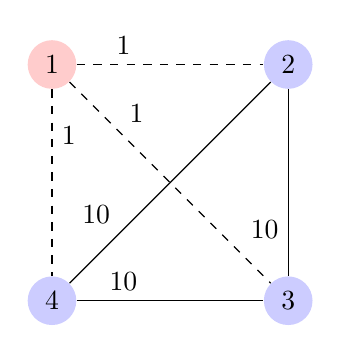
\begin{tikzpicture}[node distance=3cm]
        \node[circle,fill=red!20] (1) at (0,1.5) {1};
        \node[circle,fill=blue!20, right of=1] (2) {2};
        \node[circle,fill=blue!20, below of=1] (4){4};
        \node[circle,fill=blue!20, below of=2] (3) {3};

        \foreach \from / \to in {1/2,1/3,1/4}
            \path (\from) edge[dashed, near start, auto] node{$1$} (\to);

        \foreach \from / \to in {4/2,4/3,3/2}
            \path (\from) edge[near start, auto] node{$10$} (\to);
    \end{tikzpicture}
	}
	\qquad\qquad
	\subfigure[$W_{\{5,6,7,8\}(5)} > 0$]{
    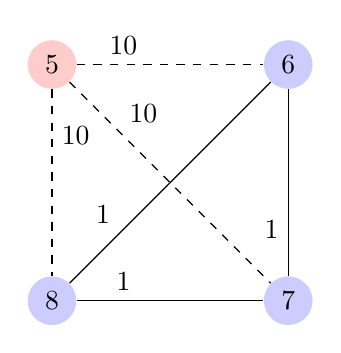
\begin{tikzpicture}[node distance=3cm]
        \node[circle,fill=red!20] (1) at (0,1.5) {5};
        \node[circle,fill=blue!20, right of=1] (2) {6};
        \node[circle,fill=blue!20, below of=1] (4){8};
        \node[circle,fill=blue!20, below of=2] (3) {7};

        \foreach \from / \to in {1/2,1/3,1/4}
            \path (\from) edge[dashed, near start, auto] node{$10$} (\to);

        \foreach \from / \to in {4/2,4/3,3/2}
            \path (\from) edge[near start, auto] node{$1$} (\to);
    \end{tikzpicture}
	}
    \caption{Rappresentazione della similarità: i nodi $\{2,3,4\}$ sono altamente simili tra loro. Se si tenta di aggiungere il vertice 1 che è dissimile dalla similarità interna dell'insieme $\{2,3,4\}$ allora la similarità complessiva del nuovo insieme $\{1,2,3,4\}$ diminuisce i.e. $W_{\{1,2,3,4\}}(1) < 0$. Nel secondo caso il vertice 5 è altamente similare ai nodi $\{6,7,8\}$ di conseguenza aggiungendolo all'insieme la similarità complessiva aumenta i.e. $W_{\{5,6,7,8\}}(5) > 0$.}
\end{figure}

\newpage

È stata dunque definita una misura che descrive cosa comporta (in termini di similarità) l'aggiunta o la rimozione di un nodo. Questo porta alla definizione di \emph{insiemi dominanti}.

\begin{mydef}[Insieme Dominante]
	Un sottoinsieme di vertici non vuoto $V \subseteq V$ tale che $W(T) > 0$ per ogni insieme non vuoto $T \subseteq S$ è detto \textbf{dominante} se:
	\begin{enumerate}
		\item $W_S(i) > 0, \forall i \in S$ (omogeneità interna)
		\item $W_{S \cup \{i\}}(i) < 0, \forall i \not\in S$ (disomogeneità esterna)
	\end{enumerate}
\end{mydef}
L'insieme dominante è dunque un insieme di vertici massimalmente coesi tra loro e questa definizione corrisponde con quella di cluster.

\begin{figure}[h!]
    \centering
	
    \begin{tikzpicture}[node distance=3cm]
        \node[circle,fill=blue!20] (1) at (0,0) {1};
		
        \node[circle,fill=blue!20, below left of=1] (2) {2};
        \node[circle,fill=blue!20, below right of=1] (3) {3};
        
        \node[circle,fill=blue!20, below of=2] (4) {4};
        \node[circle,fill=blue!20, below of=3] (5) {5};

        \foreach \from / \to / \label in {1/2/10,1/3/15,1/4/60,1/5/70}
            \path (\from) edge[near start] node{$\label$} (\to);
			
        \foreach \from / \to / \label in {2/4/25,2/5/20}
            \path (\from) edge[near start] node{$\label$} (\to);

        \foreach \from / \to / \label in {3/4/25,3/5/90}
            \path (\from) edge[near start] node{$\label$} (\to);

		\path (4) edge[auto] node{5} (5);
		\path (2) edge[auto] node{20} (3);

		\begin{pgfonlayer}{background}    % select the background layer
			\fill[gray!20] plot coordinates {(1) (3) (5)};
	    \end{pgfonlayer}

    \end{tikzpicture}
	\caption{L'insieme $\{1,3,5\}$ è dominante.}
\end{figure}
Questa nuova formulazione di cluster è stata concepita per poter sfruttare tecniche sulla teoria dei giochi. Il ponte che collega gli insiemi dominanti con la teoria dei giochi è dato dal seguente teorema:

\begin{thm}[Torsello, Rota Bulò, Pelillo 2006]
	Strategie evolutionary stable (ESS) di un problema di clustering con matrice di affinità $A$ sono in corrispondenza uno-a-uno con gli insiemi dominanti.
\end{thm}

Si tratta di una generalizzazione del teorema di Motzkin-Strauss.

% subsection definizione_insieme_dominante (end)
% section insiemi_dominanti (end)
% chapter clustering (end)




















